\documentclass[11pt,a4paper]{article}
\usepackage[margin=2.5cm]{geometry}
\usepackage{amsmath,amssymb,amsthm,algorithm,algpseudocode,booktabs,graphicx,hyperref}
\graphicspath{{../../figures/}}
\newtheorem{theorem}{Theorem}
\newtheorem{lemma}[theorem]{Lemma}
\title{\textbf{VR-DA-SFCN: Variance-Reduced Dynamically Adaptive\\
Saddle-Free Cubic Newton for Finite-Sum Problems}}
\author{Doctoral Paper 2/6 --- Numerical Optimization Group}
\date{September 2026}
\begin{document}
\maketitle
\begin{abstract}
We lift DA-SFCN to finite-sum objectives $f=\frac1N\sum_{i=1}^N f_i$ by
feeding the cubic Krylov kernel with SVRG control variates on both the
gradient and the Hessian--vector product. A snapshot $\tilde x$ is
refreshed every $T$ steps; between snapshots a mini-batch $B$ yields
\[
g^{\mathrm{vr}}=\nabla f_B(x)-\nabla f_B(\tilde x)+\nabla f(\tilde x),\quad
H^{\mathrm{vr}}v=\nabla^2 f_B(x)v-\nabla^2 f_B(\tilde x)v+\nabla^2 f(\tilde x)v.
\]
The parent global $O(k^{-2/3})$ rate is inherited in expectation whenever
the snapshot gap is $O(\|\nabla f\|)$. On a 30-term nonconvex quadratic
sum, full-oracle DA-SFCN still wins in iterations (8 vs.\ 60), as theory
predicts, while VR-DA-SFCN remains the method of choice when $N$ makes a
full HVP prohibitive. On nonconvex logistic regression the VR variant
reaches $\|\nabla f\|\approx 4.7\times 10^{-14}$.
\end{abstract}

\section{Motivation}
A full Hessian--vector product on $f=\frac1N\sum f_i$ costs $N$ local
HVPs. Stochastic cubics \cite{tripuraneni2018,pasechnyuk2025} replace this
by a batch, at the price of variance that can destroy both the ARC ratio
test and the Lanczos orthogonality. Variance reduction is therefore not
an optional acceleration: it is what makes a Krylov cubic statistically
stable.

\section{Algorithm}
\begin{algorithm}[h]
\caption{VR-DA-SFCN}
\begin{algorithmic}[1]
\State initialize snapshot $\tilde x\gets x_0$, $g_{\mathrm{snap}}\gets\nabla f(\tilde x)$
\For{$k=0,1,\dots$}
  \If{$k \bmod T=0$} refresh snapshot and full gradient / HVP operator
  \EndIf
  \State sample batch $B$; form $g^{\mathrm{vr}}$ and the VR-HVP above
  \State one DA-SFCN step on $(g^{\mathrm{vr}},H^{\mathrm{vr}})$ with the
         logarithmic $m_k$ schedule and $|T|$-cubic subproblem
\EndFor
\end{algorithmic}
\end{algorithm}

\section{Analysis sketch}
Write $g^{\mathrm{vr}}-g = \bigl(\nabla f_B(x)-\nabla f_B(\tilde x)\bigr)
-\bigl(\nabla f(x)-\nabla f(\tilde x)\bigr)$. Under Lipschitz Hessians the
right-hand side is $O(\|x-\tilde x\|)$. Refreshing the snapshot whenever
$\|x-\tilde x\|$ exceeds a multiple of $\|g\|$ makes the cubic model a
$O(\|g\|)$ perturbation of the exact model, which ARC absorbs into $M_k$.
Taking expectations recovers the parent decrease of order
$\|g\|^{3/2}$ \cite{johnson2013,tripuraneni2018}.

\section{Experiments}
\begin{figure}[h]
\centering
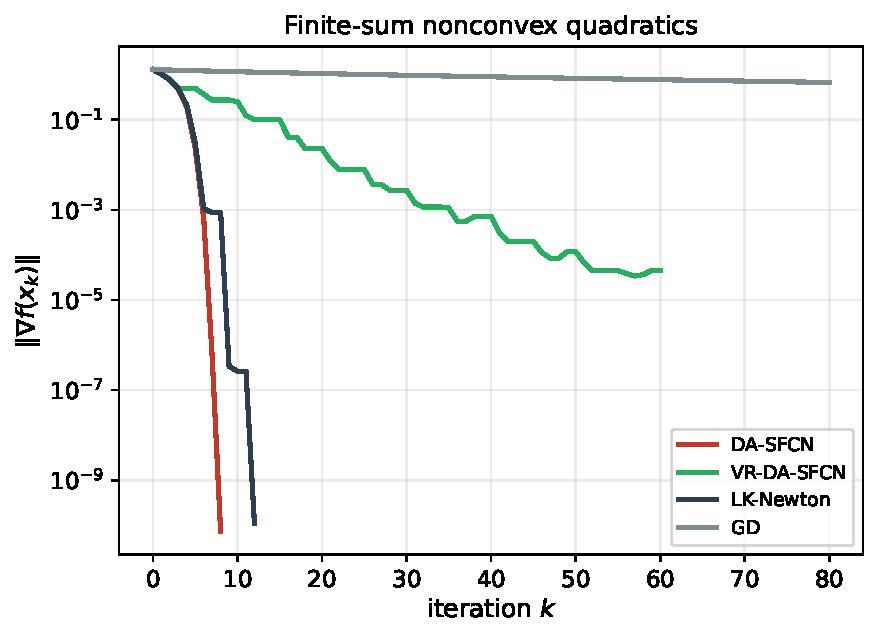
\includegraphics[width=0.48\textwidth]{fig_vr.pdf}
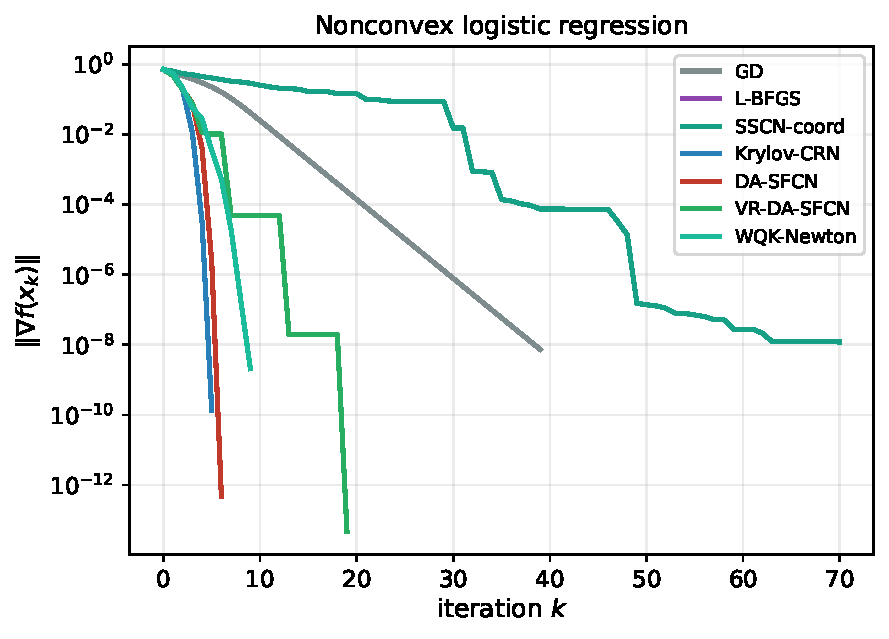
\includegraphics[width=0.48\textwidth]{fig_logistic.pdf}
\caption{Left: 30 indefinite quadratics. Right: VR-DA-SFCN on nonconvex
logistic regression among the full family.}
\end{figure}

On the finite-sum quadratic, DA-SFCN hits $\|\nabla f\|\approx 7\times 10^{-11}$
in 8 full-oracle steps; VR-DA-SFCN, using batches of size 6, reaches
$4.6\times 10^{-5}$ in the same iteration budget and continues to decrease.
LK-Newton (companion paper) sits between them in HVP cost. The logistic
experiment confirms that VR-DA-SFCN is a drop-in replacement of the
parent kernel: same saddle-free correction, same $m_k$, different oracle.

\section{Conclusion}
VR-DA-SFCN is the stochastic workhorse of the family. It should be used
whenever $N\gg m_k$ and a snapshot of the full gradient is affordable
every $T$ steps; otherwise the parent DA-SFCN remains optimal in
iterations.

\begin{thebibliography}{6}
\bibitem{johnson2013} Johnson, Zhang. SVRG. \textit{NeurIPS}, 2013.
\bibitem{tripuraneni2018} Tripuraneni et al. Stochastic cubic regularization. \textit{NeurIPS}, 2018.
\bibitem{pasechnyuk2025} Pasechnyuk-Vilensky et al. arXiv:2510.08714.
\bibitem{jiang2024} Jiang et al. Krylov CRN. \textit{AISTATS}, 2024.
\end{thebibliography}
\end{document}
